\documentclass[a4paper, titlepage, twoside]{article}
%\usepackage[fontset=windows]{ctex}
\usepackage{ctexcap}
\usepackage{mathrsfs}
\usepackage{fancyhdr}
\usepackage{latexsym, amsfonts, amssymb, amsmath,  amsthm}
\usepackage{amsopn, amstext, amscd,pifont}
\usepackage{amssymb,bm, cite, color}
\usepackage{thmtools}
\usepackage{extarrows}
\usepackage{mathdots}
%\usepackage[normalem]{ulem}
\usepackage[all]{xy}
\usepackage{enumitem}
\usepackage{graphicx}
\usepackage{titlesec}
\usepackage{titletoc}
\usepackage{zhnumber}
\usepackage{etoolbox}
\usepackage{tikz}
\usepackage{stmaryrd} %---This is a package for writing things on long arrows
\usepackage[a4paper, left=2cm, right=2cm, top=2.5cm, bottom=2.5cm]{geometry}
%----------------the 'geometry' package doesn't seem to set dimensions right


%------------------The following segment redefines \cleardoublepage to get rid
%------------------of headers and footers on the empty even numbered pages
\makeatletter
\renewcommand*{\cleardoublepage}{\clearpage\if@twoside \ifodd\c@page\else
\hbox{}%
\thispagestyle{empty}%
\newpage%
\if@twocolumn\hbox{}\newpage\fi\fi\fi}
\makeatother
%----------------It stops here---------------------------------------------
\pretocmd\section{\cleardoublepage}{}%
  {\errmessage{Patching \noexpand\section failed}}
%-----The above command forces each section to start on odd numbered pages

%-----The following uses the 'titlesec' and 'titletoc' packages to set the
%-----format of section titles and their format in the TOC
\renewcommand\thesection{\zhnum{section}}
\renewcommand{\thesubsection}{\arabic{subsection}}
\titleformat{\section}{\normalfont\Large\bfseries\centering}{\thesection}{1em}{}
\titlecontents{section}[5em]{}{\contentslabel[\large\bfseries\kaishu\hfill\thecontentslabel\hspace*{1em}]{5em}\large\bfseries\kaishu}{\hspace*{-5em}}{\hfill\contentspage}
\titlecontents{subsection}[7em]{}{\contentslabel{1.5em}}{\hspace*{-1.5em}}{\titlerule*[1pc]{.}\contentspage}
%----It stops here--------------------------------------------------------



% Adjusting the theorem-environment style
\declaretheorem[name=定理,%
	postheadhook=\normalfont\slshape,%
	numbered=no]{theorem}
\declaretheorem[name=例子,%
	postheadhook=\normalfont\slshape,%
	numbered=no]{example}
\declaretheorem[name=推论,%
	postheadhook=\normalfont\slshape,%
	numbered=no]{corollary}
\declaretheorem[name=命题,
	postheadhook=\normalfont\slshape,%
	numbered=no]{proposition}
\declaretheorem[name=定义,
	postheadhook=\normalfont\slshape,%
	numbered=no]{definition}
\declaretheorem[name=注记,
	postheadhook=\normalfont\slshape,%
	numbered=no]{remark}
\declaretheorem[name=引理,
	postheadhook=\normalfont\slshape,%
	numbered=no]{lemma}
\declaretheorem[name=性质,%
	postheadhook=\normalfont\slshape,%
	]{xingzhi}
\newenvironment{jie}{\noindent{\bf 解:}}{\hfill$\blacksquare$\par}
% Theorem-environment style adjustment stops here



%\renewcommand{\figurename}{\tiny{\bfseries 图表}}
\renewcommand{\proofname}{\bfseries 证明}
%\renewcommand{\contentsname}{目\quad 录}
%\renewcommand{\refname}{\small\centering 参考文献}
% Numbering the equations within sections
\numberwithin{equation}{section}
\allowdisplaybreaks
% -----------------------------------------------------------
\linespread{1.5}

\CJKsetecglue{\hskip 0.15em plus 0.05em minus 0.05em} %--调整正英文间距







\begin{document}
\zihao{-4}
\pagestyle{empty}
\renewcommand{\labelenumi}{(\arabic{enumi}).}




\title{\bf\kaishu 2015-2016第二学期\\ 高等数学教案}
\author{Someone Someone}
\date{听课班级:2015某某某某某某1班}
\maketitle

\cleardoublepage
\tableofcontents
\cleardoublepage

\pagestyle{fancy}
\lhead{\tiny\kaishu 2015某某某某某某1班}
\fancyhead[OC]{\tiny\kaishu \nouppercase\leftmark}
\fancyhead[EC]{\tiny\kaishu \nouppercase\rightmark}
\rhead{\tiny\kaishu 2016年2月至2016年7月}
\cfoot{\small\kaishu \thepage}
\setcounter{page}{1}

\section{一元函数微积分复习和微分方程}
\subsection{教学目的}
学生能够验证一个函数是不是一个常微分方程的解. 
\subsection{教学重点于难点}
常微分方程和它们的解的含义. 

\subsection{教学内容与过程}

说先花半个小时左右的时间将上一学期所学的内容整体复习一遍. 

\ \par
微积分理论在数学的其他分支,在物理学问题当中,工程问题当中,某些化学问题,
某些社会科学问题当中都有相当广泛的应用. 举大家非常熟悉的例子,假设在直线上
有一个质量为$m$的质点,
它在时间$t$的时候所在的位置为$x(t)$, 我们又知道这个质点在时间
$t$的时候的受力是$F(t)$.
那么为了求出质点的运动规律,我们可以使用牛顿第一定律,
我们有
$$ m\frac{d^2x(t)}{dt^2}=mx''(t)=F(t).\eqno(1)$$
所以该质点的运动规律$x(t)$满足方程$(1)$. 那么这个函数$x(t)$应该怎么找呢?
我们由$(1)$得
$$ x''(t)= \frac{F(t)}{m}.$$
所以$x'(t)$作为$x''(t)$的原函数应该有
$$ x'(t) = \int mF(t)\,dt.$$
然后再由$x(t)$是$x'(t)$的原函数,我们可以得到:
$$ x(t) = \int \left(\int mF(t)\,dt\right)\,dt. \eqno(2)$$
所以本质上我们只要作两次的积分就可以求出$x(t)$这个函数关于时间$t$的表达式. 

\begin{definition}
	我们把一个表示自变量、取决于自变量的未知函数和这些未知函数的导数
	的方程称为一个{\bf 微分方程}. 当自变量的个数是一个时,我们就称该
	微分方程为一个{\bf 常微分方程}. 在我们这门课里,我们一般只考虑
	常微分方程. 在不引起混淆的情况下,我们将“微分方程”、“常微分方程”、
	和“方程”看成是同一个概念. 在微分方程当中出现的未知函数的导数的最
	高阶称为该方程的{\bf 阶}. 有时候我们将微分方程中未知函数的个数
	称为该微分方程的{\bf 元}. 
\end{definition}

上面的$(1)$式就是一个一元二阶常微分方程的例子. 一般地,我们可以将一个$n$阶常
微分方程写成
$$ F(x, y, y', \ldots, y^{(n)})=0, \eqno(3)$$
其中$x$是自变量,$y$是关于$x$的函数,$F$是某一个多元函数. 


\begin{definition}
	对于一个常微分方程$(3)$, 如果定义在区间$I$上的函数$y=\phi(x)$具有
	$n$阶导数而且在区间$I$上
	$$ F(x, \phi(x), \phi'(x), \ldots, \phi^{(n)}(x))\equiv 0,$$
	那么我们就称$y=\phi(x)$是$(3)$在区间$I$上面的一个解. 
\end{definition}

我们下面在来看一个具体一点的例子. 

\begin{example}[P297, 例2]
	列车在平直路上以$20m/s$的速度行驶,当制动时列车获得加速度$-0.4m/s^2$.
	问开始制动后多少时间列车才能停住以及列车在这段时间里行驶的路程. 
\end{example}
\begin{jie}
	假设列车在时间$t$时所行驶的路程为$s=s(t)$, 那么我们有
	$$ s''(t) = -0.4.\eqno(4)$$
	所以$s'(t)=-0.4t+C_1$, $C_1\in \mathbb{R}$. 从而
	$$ s(t) = \int (-0.4t+C_1) \,dt = -0.2t^2 + C_1t + C_2, \quad C_1,
	C_2\in \mathbb{R}. \eqno(5)$$
	又因为我们有初始条件$s(0)=0$, $s'(0)=20$. 所以
	$$ \begin{cases} C_2&=0,\\ C_1&=20.\end{cases}.$$
	所以$s(t)=-0.2t^2 +20t$, 这时候$t\geq 0$而且有一个上限$t_0>0$, 这里
	的$t_0$就是列车从开始制动到停止所需要的时间,此时列车速度是零,
	所以$s'(t_0)=0$, 即$-0.4t_0 + 20=0$, 解得$t_0=50$. 同时$s(t_0)=500$.

	所以列车需要$50$秒才能完全停止,在这$50$秒钟内列成行驶了$500m$.
	列车停止. 
\end{jie}

在这道例题当中,我们利用积分的方法就原函数从而解了微分方程,得到一个解$(5)$式. 
由我们前面的积分学的内容,$(5)$式给出了所有的$(4)$式的解. 我们称$(5)$式为$(4)$
式的通解. 


\section{可分离变量的微分方程}
\subsection{教学目的}
学生能够解决一些简单的可
分离变量的常微分方程. 
\subsection{教学重点与难点}
可分离变量的微分方程的解法. 
\subsection{教学内容与过程}
\begin{definition}
	假设
	$$ F(x,y, y', y'', \ldots, y^{(n)})=0$$
	是一个以$x$为自变量的以$y$为未知函数的$n$阶微分方程. 如
	果$y=\phi(x,C_1,\ldots,
	C_n)$是一个含有$n$个独立的自由常数$C_1,\ldots, C_n$的解,那么我们
	称其为该微分方程的一个{\bf 通解}. 
	在通解当中确定了任意常数以后得到的一个解
	就称为该微分方程的一个{\bf 特解}. 
\end{definition}
\begin{remark}
	我们这本书上定义的通解的概念并不是指所有的解. 这是一个比较不幸
	的情形. 一般情况下,在微分方程当中通解是在线性微分方程当中的一个
	概念,而对于一般的微分方程,比较少用这个概念. 通解不包含所有的解的
	情形,例如,先面我们会学到
	$$ y'=y, \quad y=y(x)$$
	的所有的解都可以表示成为$y=Ce^{x}, C\in \mathbb{R}$. 这个表达式
	是一个通解. 但是我们也可以有$y=e^Ce^x, C\in \mathbb{R}$, 这个解
	按照我们的定义也是一个通解. 但是它并没有包括零解和负解. 

	所以一般情况下,我们遇到的题目如果是叫你找到一个微分方程的通解,
	那么它的意思是让你找到一个据有$n$个独立的参数的解,而不是所有的解. 

	对于一般的微分方程,要找到所有的解并不是一件容易的事. 
\end{remark}

\begin{example}
比如上面我们的$(5)$式就是通解,而确定了通解中的$C_1,
C_2$之后得到的$s(t)=-0.2t^2 +20t$就是一个特解. 
\end{example}

形如上面的例子中的,给出一个
常微分方程以后又给出一些初始条件$y|_{x=x_0}=y_0$, $y'|_{x=x_0}=y'_0$, 使得我们
能够确定出的解的问题一般称为一个{\bf 初值问题}. 典型的一阶方程的初值问题可以
写成
$$ \begin{cases}  y'=f(x,y),\\  y|_{x=x_0}=y_0.\end{cases}
$$
典型的二阶方程的初值问题可以写成
$$ \begin{cases}  y''=f(x,y,y'),\\  y|_{x=x_0}=y_0, y'|_{x=x_0}=y'_0.
\end{cases}
$$
微分方程的解的图形通常称为该微分方程的一条{\bf 积分曲线}. 上面的二阶微分
初值问题实际上就是求微分方程的通过点$(x_0,y_0)$而且斜率为$y'_0$的积分曲线. 


一般的微分方程的求解是比较复杂的问题,当然并不是所有的微分方程都是有解的. 
很多情况下即使一个微分方程有解,解也不能用分段初等函数来表示. 我们在这一章
当中会学到一些常见的可以写出显示解的常微分方程. 

回到刚才我们的微分方程$(1)$, 如果我们的质点是一支火箭,那么随着时间的不同,
火箭上面的燃料的量也发生了变化,那么质点的质量又是$t$的函数$m(t)$, 有的时候
我们又只知道力$F$的作为位移和时间的函数
(例如它在不同的地点受到的万有引力又不一样),这个时候方程就稍微复杂一点:
$$ m(t)x''(t)=F(t, x).$$
但我们还是可以用微分方程的理论来研究它. 

\begin{example}[P300, 例3]
	根据授课剩余时间来决定是否讲解. 
\end{example}

\begin{example}[P301, 例4]
	根据授课剩余时间来决定是否讲解. 
\end{example}



下面我们就开始讨论一类比较容易求解的一阶常微分方程,叫作“可分离变量的常微分方程”. 
注意到我们前面的几个微分方程的例子都是可以直接用积分的方法得到解的,可以想像
一般情况下直接作积分的话是行不通的,例如
$$ y'=y$$
这个方程,直接积分我们就不知道该怎么做,因为我们发现$y=\int y\,dx$的被积函数
当中还是有未知函数. 但是稍微变化一下我们实际上是可以求出它的解的. 

我们不妨先假设$y\neq 0$, 那么我们有
$$ \frac{1}{y}y'=1.$$
这个时候两边都是关于$x$的函数,所以我们可以两边同时对$x$积分:
$$ \int \frac{1}{y} y' dx = \int 1 dx = x+C.$$
所以我们只需要解决左边的积分就可以了. 因为我们知道$y$是关于$x$的一个可导函数,
所以利用不定积分的第一换元公式就有:
$$ \int \frac{1}{y} y'dx=\int \frac{1}{y} dy.$$
上式的右边是一个纯粹关于$y$的积分,所以我们有
$$ \int \frac{1}{y}y'dx=\ln|y|+C.$$
因此我们原来的微分方程可以通过两边同时对$x$积分得到
$$ \ln|y|=x+C, \quad C\in \mathbb{R},$$
其中我们把两边的积分后得到的常数合并成为一个自由常数$C$. 
这样以后两边再同时取以$e$为底的指数,得到
$$ |y|=e^{x+C}\implies y=\pm e^C e^x, \quad C\in \mathbb{R}.$$
这便是$y'=y$的一个通解. 我们上面的做法是假设了$y\neq 0$, 所以如果我们想要
得到所有的解的话,还要讨论$y=0$的情况. 对于我们这个方程,可以证明如果存在
一个$x_0$使得$y(x_0)=0$, 那么$y\equiv 0$. 所以我们可以用一个通解
$$ y=Ce^x, \quad C\in \mathbb{R},$$
将所有的解都表示出来. 

上面我们的计算过程很多时候我们都是采用如下的方式来写:
由$y'=y$, 假设$y\neq 0$, 则有
$$ \frac{1}{y}\frac{dy}{dx} = 1.$$
两边同乘以$dx$, 则有
$$ \frac{1}{y}dy = 1 dx.$$
此时两边同时对$x$进行积分,又由于$y$是$x$的函数,所以左边相当于对
$y$的积分:
$$ \int \frac{1}{y}dy = \int \frac{1}{y}y'dx = \int 1 dx.$$
所以我们有
$$ \ln|y| = x + C, \quad C\in \mathbb{R}.$$
所以$y=\pm e^C e^x$, 又因为$y\equiv 0$也是原方程的解,所以将$\pm e^C$用
一个单独的常数替代,得到我们的通解是
$$ y=Ce^x, \quad C\in \mathbb{R}.$$



\begin{definition}
	如果一个方程可以写成
	$$ g(y)\frac{dy}{dx}=f(x). \eqno(7)$$
	的形式,那么我们就称该微分方程为一个{\bf 可分离变量}的微分方程. 
	$(7)$式通常又写成$g(y)dy=f(x)dx$. 
\end{definition}

对于$(7)$式给出的方程,由不定积分的第一种换原法我们有
$$ \int g(y)dy = \int f(x)dx,$$
也就是说我们可以对$(7)$式两边同时作积分,仍然得到一个恒等式. 这时候如果
我们能够分别求出两边的积分,设$\Phi(y)$为$g(y)$关于$y$的一个原函数, 
$\Psi(x)$为$f(x)$的一个
原函数, 
则我们得到$(7)$的隐式解
$$ \Phi(y)=\Psi(x)+C, \quad C\in \mathbb{R}.$$

\begin{definition}
	对于一个微分方程,如果我们有关于$x,y$的一个隐式关系
	$$ G(x,y)=0,$$
	满足在每一个恰当的局部$G(x,y)$所确定的$y=\phi(x)$是该微分
	方程的一个解,那么我们就称$G(x,y)=0$为该方程的一个{\bf 隐式解}. 
\end{definition}


\begin{example}[P328, 例1]
	求以下微分方程的一个通解:
	$$ \frac{dy}{dx}= 2xy.$$
\end{example}
\begin{jie}
	由原来的微分方程得:
	$$ \frac{1}{y} dy = 2x dx,$$
	所以两边同时积分得
	$$ \ln|y| = x^2 + C,\quad C\in \mathbb{R}.$$
	这就是该微分方程的一个隐式通解. 我们可以将它更进一步地化为
	$$ |y| =e^Ce^{x^2} \implies y=\pm e^C e^{x^2}, \quad C\in
	\mathbb{R}.$$
	由于$y\equiv 0$也是原方程的解,所以我们有通解:
	$$ y=Ce^{x^2}, \quad C\in \mathbb{R}.$$
\end{jie}


\subsection{作业}

P326, 习题6-1, 2(3).

P335, 习题6-2, 1(1), 4(1).


\subsection{教学反思}


\section{一阶线性微分方程}
\subsection{教学目的}
学生能够解简单的一阶线性微分方程. 
\subsection{教学重点与难点}
一阶线性微分方程的解法. 
\subsection{教学内容}

首先对前面讲的内容进行回顾. 

\ \par
接下来我们来研究比可分离变量的微分方程稍微复杂一点的一阶线性微分方程. 

\begin{definition}
	假设$P(x), Q(x)$为关于$x$的已知函数,那么关于未知函数$y=y(x)$
	的一阶微分方程
	$$ y' + P(x)y=Q(x) \eqno(1)$$
	称为一个{\bf 一阶线性微分方程}. 其中“线性”的意思是对于$y'$与$y$是
	线性的. 

	当$Q(x)\equiv 0$时,我们称方程$(1)$是{\bf 齐次}的;当$Q(x)\not\equiv 0$
	时我们称方程$(1)$是{\bf 非齐次}的. 
\end{definition}

由我们的定义,一个齐次的一阶线性微分方程
$$ y' + P(x)y=0 \eqno(2)$$
实际上是一个可分离变量的微分方程,我们可以用上次课讲到的方法来求解. 我们可以
将$(2)$式化成
$$ y'=-P(x)y \implies \frac{1}{y}dy=-P(x)dx.$$
所以
$$ \ln|y| = -\int P(x)\,dx.$$
如果我们令$I(x)$为$P(x)$的一个原函数,那么
$$ \int P(x) \,dx = I(x)+C, \quad C\in\mathbb{R}.$$
所以
$$ y= \pm e^{-\int P(x)\,dx}=\pm e^C e^{-I(x)}.$$
所以$(2)$式的通解为
$$ y= C e^{-I(x)}, \quad C\in\mathbb{R}. \eqno(3)$$

我们接下来证明一个结论

\begin{theorem}
	在任意给定的一个开区间上面,$(3)$式恰好给出了$(2)$式的所有解. 
\end{theorem}
\begin{proof}
	首先,对于任意的$y=y(x)$满足$(3)$式, 我们有
	$$ y'=Ce^{-I(x)}I'(x)=y(x)P(x)\implies y'-P(x)y=0.$$
	所以满足$(3)$式的$y$都是$(2)$式的解. 

	其次,如果$y_1=\phi(x)$式$(2)$式的一个解. 那么我们考虑
	\begin{align*}
		\frac{d}{dx}\left(\frac{y_1}{e^{-I(x)}}\right)&=
		\frac{d}{dx}\left(y_1e^{I(x)}\right) \\
			&=
			y_1'e^{I(x)}+y_1e^{I(x)}I'(x) \\
			&=
			e^{I(x)}(y_1'+P(x)y_1)\\
			&\equiv 0.
	\end{align*}
	所以在一个开区间上面$y_1/e^{-I(x)}$是一个常数,即$y_1$必
	形如$Ce^{-I(x)}$.
\end{proof}

\begin{remark}
	因为我们讨论微分方程的解的时候强调的是在某个开区间上面的解,
	所以如果我们讨论的定义域不是开区间的话,那么满足方程的函数
	的表达式通常情况下会
\end{remark}


所以对于一阶齐次线性微分方程$(2)$, 它的通解是很容易求的. 下面我们由此来讨论
非齐次的$(1)$式的解. 我们采用所谓的{\bf 常数变易法}. 我们假设$y_1$是$(1)$式
的一个解,那么我们令
$$ C(x):=y_1e^{I(x)}, $$
则我们有
$$ y_1= C(x)e^{-I(x)}.\eqno(4)$$
也就是说我们可以将$(3)$式中的常数$C$看成是一个关于$x$的函数, 那么任何一个
非齐次方程的解都可以表示成$(4)$式. 下面我们来求$C(x)$因该满足的条件. 因为我们
假设了$y_1$是$(1)$式的解,所以我们有
$$ y_1' +P(x)y_1 = Q(x),$$
所以我们将$(4)$式代入,得到
$$ C'(x)e^{-I(x)} - C(x) e^{-I(x)} P(x) + P(x) C(x) e^{-
I(x)} = Q(x),$$
即
$$ C'(x)e^{-I(x)} = Q(x),$$
所以
$$ C'(x) = Q(x)e^{I(x)}.$$
如果我们令$u(x)$为$Q(x)e^{I(x)}$的一个原函数,那么我们有
$$ C(x) = u(x)+C, \quad C\in \mathbb{R}.$$
所以
$$ y_1 = (u(x)+C)e^{-I(x)}, \quad C\in\mathbb{R}.$$
这个就是我们的$(1)$式的通解. 

因为引入新的函数$I(x)$, $u(x)$等使得我们不方便看清它们之间的关系,有时候我们
也用比较不严格的记法:
$$ y=e^{-\int P(x)dx} \left(\int Q(x) e^{\int P(x)dx}dx+C\right), \quad C\in
\mathbb{R}, \eqno(5)$$
其中积分符号``$\int$''表示的是取某一个特定的原函数,而不是取所有的原函数. 

\begin{theorem}
	$(5)$式是一阶线性非齐次微分方程$(1)$式的通解. 而且在某一给定的
	区间上面,$(5)$式恰好给出了$(1)$式的所有解. 
\end{theorem}
\begin{proof}
	这个定理的证明我们在下次课再给出. 
\end{proof}

我们下面来看几个例子. 


\begin{example}[P337, 例1]
	求解微分方程:
	$$ y' -\frac{2y}{x+1} = (x+1)^{5/2}.$$
\end{example}
\begin{jie}
	我们注意到要使原来的方程式是有意义的,应该有$x+1>0$. 所以我们下面
	可以假设$x+1>0$. 

	这个时候令
	$$ P(x)=\frac{-2}{x+1}, \quad Q(x)=(x+1)^{5/2}, $$
	则
	$$ \int P(x) dx = -\int \frac{2}{x+1}dx = -2\ln(x+1) + C_1, \quad
	C_1\in \mathbb{R},$$
	所以我们取$I(x)$为$P(x)$的一个原函数,
	$$ I(x):=-2\ln(x+1).$$
	此时
	\begin{align*}
		\int Q(x) e^{I(x)}dx &= \int (x+1)^{5/2}(x+1)^{-2}dx =\int
	(x+1)^{1/2}dx \\
	&=\frac{2}{3}(x+1)^{3/2}+C_2, \quad C_2\in \mathbb{R}.
	\end{align*}
	所以我们的通解是
	\begin{align*}
		y &= e^{-I(x)}\left(\frac{2}{3}(x+1)^{3/2}+C\right) \\
		  &=(x+1)^2\left(\frac{2}{3}(x+1)^{3/2}+C\right), \quad C\in
		\mathbb{R}.
	\end{align*}
\end{jie}


\begin{example}[P341, 习题6-3, 2(1)]
	求下面初值问题的解:
	$$ y'-y\tan x =\sec x, \quad y|_{x=0}=0.$$
\end{example}
\begin{jie}
	对于初值问题,我们通常只关心它在某一包含初值点的小开区间上面的
	一个解,因此如果需要的化,我们总可以假设我们求解的时候,$x$和
	$0$是足够靠近的. 

	令
	$$ P(x) := -\tan x, \quad Q(x):= \sec x, $$
	那么我们有
	$$ \int P(x) dx = -\int \tan x dx = \int \frac{d\cos x}{\cos x}, $$
	我们可以假设$x\in (-\pi/2, \pi/2)$, 那么这个时候$\cos(x)>0$,  所以
	$$ \int P(x)dx=\ln(\cos x) + C_1, \quad C_1 \in \mathbb{R}.$$
	我们取$I(x)=\ln(\cos x)$, 则
	$$ \int Q(x) e^{I(x)} = \int \sec x \cos (x) dx =x + C_2, \quad C_2\in
	\mathbb{R}, $$
	所以在区间$(-\pi/2, \pi/2)$上面,我们的微分方程的通解是
	$$ y= \sec x ( x + C), \quad C\in \mathbb{R}.$$

	由初值条件$y(0)=0$知道, $C=0$, 所以我们的初值问题的解为
	$$ y=x\sec x, \quad x\in (-\pi/2, \pi/2).$$
\end{jie}

\subsection{作业}

P341, 习题6-3, 1(3), 2(2).
\subsection{教学反思}




\section{二阶常系数齐次线性微分方程}
\subsection{教学目的}
学生能够解三种类型的二阶常系数齐次线性微分方程. 
\subsection{教学重点与难点}
二阶常系数齐次线性微分方程和它们的特征方程特征根的关系. 
\subsection{教学内容}

我们前面学习了两种比较简单的类型的微分方程的求解问题,一种是可分离变量
的常微分方程,另一种是一阶线性常微分方程. 这两种方程的解法都比较简单. 
我们先来回顾一下一阶线性常微分方程的通解的形式. 

如果我们的一阶线性常微分方程是一个齐次的方程
$$ y' + P(x)y=0,$$
那么我们证明了在某一个区间上面,它的所有的解恰好就是
$$ y= Ce^{-\int P(x) dx}, \quad C\in \mathbb{R}.$$
另外一方面,如果我们的方程是非齐次的:
$$ y' + P(x)y =Q(x), \eqno(1)$$
那么我们有一个定理说明了它的在某一个开区间上面的解恰好就是:
$$ y=e^{-\int P(x) dx}\left(\int Q(x)e^{\int P(x)dx}dx+C\right), \quad C\in
\mathbb{R}. \eqno(2)$$
这个公式可能有一些同学觉得不是很好记. 这里再介绍一种比较快速的推导方法:
我们令
$$ J(x):= e^{\int P(x)dx}.$$
注意到此时我们有
$$ J'(x)=e^{\int P(x)dx}P(x) =J(x)P(x).$$
在$(1)$式两边同乘以$J(x)$得到
$$ J(x)y' + J(x)P(x)y = Q(x)J(x).$$
注意到上面这个等式的左边恰好是一个乘积的倒数,我们有
$$ (J(x)y)' = Q(x)J(x).$$
所以
$$ J(x)y = \int Q(x)J(x) + C, \quad C\in \mathbb{R},$$
所以我们就得到通解:
$$ y= J(x)^{-1} \left( \int Q(x)J(x) + C\right), \quad C\in \mathbb{R}.$$
将$J(x)$用$e^{\int P(x)dx}$替换回来我们就得到了$(2)$式. 上面的$J(x)$有时候
也称为是$(1)$式的{\bf 积分因子}. 


我们上次课并没有证明$(2)$式恰好是所有的解. 我们在这里给出一个证明. 

\begin{theorem}
	$(2)$式是一阶线性非齐次微分方程$(1)$式的通解. 而且在某一给定的
	区间上面,$(2)$式恰好给出了$(1)$式的所有解. 
\end{theorem}
\begin{proof}
	容易验证对于任意的实数$C\in \mathbb{R}$, $(2)$总给出了$(1)$式的
	一个解. 我们令$C=0$, 并令
	$$ y_2= e^{-\int P(x)dx} \int Q(x)e^{\int P(x)dx} dx.$$
	现在假设$y_1$式$(1)$式的一个解,那么我们有
	\begin{align*}
		y_1' + P(x)y_1 & = Q(x), \\
		y_2' + P(x)y_2 &= Q(x). 
	\end{align*}
	上面两式相减后得到
	$$ (y_1-y_2)' + P(x) (y_1-y_2)=0.$$
	有上一次课的一阶齐次线性微分方程在某个开区间$I$上的所有解的表达式,
	我们知道存在一个常数$C\in \mathbb{R}$, 满足
	$$ y_1-y_2 = Ce^{-\int P(x)dx}, $$
	即
	$$ y_1 = e^{-\int P(x)dx} \left(\int Q(x) e^{\int P(x) dx} dx +
	C\right), \quad C\in \mathbb{R}.$$
	这说明了在开区间$I$上面,$(2)$式包含了所有的解. 
\end{proof}

接下来我们来讨论二阶的齐次线性微分方程的解法. 

\begin{definition}
	假设$p, q\in \mathbb{R}$是两个已知常数,我们称形如
	$$ y'' + py' + q =0 \eqno(3) $$
	的微分方程为一个{\bf 二阶常系数齐次线性微分方程}. 这里的“齐次线性”是指
	该方程对于$y'', y', y$是“线性的”,而且都是一次的. 这里的“常系数”指的
	是关于$y'', y', y'$的系数都是关于$x$的常数,而不是变换的函数. 
\end{definition}

给定形如$(3)$式的一个方程,我们应该怎么样来找它的解呢?我们先给出“线性无关”
的函数的定义,然后再来讨论这个问题. 

\begin{definition}
	假设$y_1(x)$与$y_2(x)$是两个关于自变量$x$的函数,如果在某个开区间$I$
	上,其中任意一个都不是另一个的常数倍,那么我们称它们是{\bf 线性无关}的;
	也就是
	说,如果在$I$上,找不到$C_1\in \mathbb{R}$或者$C_2\in \mathbb{R}$满足,
	$$ y_1(x)\equiv C_1 y_2(x), \text{ 或者 } y_2(x)\equiv C_1 y_1(x), $$
	那么我们称$y_1(x)$与$y_2(x)$线性无关. 
\end{definition}

容易证明,当$y_1$与$y_2$中,$y_2\neq 0$时,$y_1$与$y_2$是线性无关的当且仅当
不存在$C\in \mathbb{R}$, 满足$y_1(x)/y_2(x)\equiv C$. 

\begin{theorem}
	假设$y_1(x)$和$y_2(x)$是方程$(3)$式的两个解,那么对于任意的实数$C_1,
	C_2$, $C_1 y_1(x) + C_2y_2(x)$都是$(3)$式的解.  
\end{theorem}
\begin{proof}
	由我们的假设,有
	\begin{align*}
		y_1 '' + py_1' + q y &= 0,  \\
		y_2 '' + py_2' + q y &= 0.
	\end{align*}
	所以将上面的第一个式子乘以$C_1$加上第二个式子乘以$C_2$就得到
	$$ (C_1y_1+C_2y_2)'' + p(C_1y_1+C_2y_2)'+q(C_1y_1+C_2y_2)=0.$$
	所以$C_1y_1(x)+C_2y_2(x)$也是$(3)$式的一个解.   
\end{proof}

下面的定理的证明比较复杂,我们略过去不讲,同学们如果有兴趣的话可以去查阅相关
资料. 

\begin{theorem}
	在给定的一个开区间上,假设$y_1(x)$与$y_2(x)$是$(3)$式的两个线性无关的
	解,那么$(3)$式的通解
	$$ y=C_1y_1(x) + C_2y_2(x), \quad C_1, C_2\in \mathbb{R},$$
	恰好给出了$(3)$式的所有的解. 
\end{theorem}

所以我们剩下的任务就是找出$(3)$式的两个线性无关的解. 数学家欧拉的观察是:对于
函数
$$ y=e^{rx}, \quad r\in \mathbb{R}, \eqno(4)$$
我们有
$$ y^{(n)} = r^{n} e^{rx}, $$
所以如果我们将$(4)$式代入$(3)$式,就得到
$$ (r^2+ pr+q) e^{rx} = 0.$$
所以由于$e^{rx}\neq 0$, 我们有
$$ r^2 + pr + q  = 0. \eqno(5)$$
所以如果$(3)$式有一个形如$(4)$式的解的话,那么$r$一定是方程$r^2+pr+q=0$的根. 

\begin{definition}
	我们将$(5)$式称为$(3)$式的{\bf 特征方程}, 将$(5)$的一个根称为是
	$(3)$式的一个{\bf 特征根}. 
\end{definition}


对于$(3)$式的解,我们可以按它的特征方程$(5)$的解的情况来讨论:
\begin{enumerate}
	\item 如果特征方程$(5)$式有两个不同的实数解,那么我们记$r_1, r_2$为
		这两个不同的特征根. 此时令
		$$ y_1(x):=e^{r_1x}, \quad y_2(x):=e^{r_2x}, $$
		那么$y_1(x)/y_2(x)=e^{(r_1-r_2)x}$. 因为我们假定$r_1\neq r_2$, 
		所以$e^{(r_1-r_2)x}$在任何一个开区间上面都不是一个常数. 所以
		在任何一个开区间上面,$y_1(x)$与$y_2(x)$都是线性无关的. 所以
		根据上面的定理,我们得到了$(3)$是在某个开区间上面的所有的解:
		$$ y= C_1 e^{r_1x} + C_2 e^{r_2x}, \quad C_1, C_2\in
		\mathbb{R}.$$
	\item 如果特征方程$(5)$式有两个相同的实根,那么我们记这个相同的实根为
		$r_1$.
		此时显然$y_1(x)=e^{r_1x}$是方程$(3)$的一个解. 但是用这种
		方法最多这能给我们一个解. 我们还需要另外一个解. 我们可以采用
		常数变易法:设$y_2(x)= u(x)e^{r_1x}$是$(3)$是的另外一个解. 
		那么将其代入$(3)$式,我们可以算出来
		$$ u(x) = Dx +E, \quad D, E \in \mathbb{R}.$$
		所以此时我们可以令$y_2(x)=xe^{r_1x}$, 这显然是与$y=e^{r_1x}$ 
		线性无关的一个解. 所以此时$(3)$式在某一个开区间上面的所有解为:
		$$ y= C_1 e^{r_1x } + C_2 xe^{r_1x}, \quad C_1, C_2\in
		\mathbb{R}.$$
	\item 如果特征方程$(5)$式没有实根,那么此时$(5)$式具有两个互相共轭的
		复根,假设这两个共轭的复根是
		$$ \alpha \pm i\beta, \quad \alpha, \beta\in \mathbb{R}. $$
		那么可以证明
		$$ y_1(x)= e^{\alpha x} \cos(\beta x), \quad y_2(x)=e^{\alpha
		x}\sin(\beta x),$$
		是$(3)$式的两个线性无关的解. 所以此时在任何一个开区间上面,$(3)$
		式的所有解是:
		$$ y= C_1 e^{\alpha x} \cos(\beta x) + C_2 e^{\alpha x}
		\sin(\beta x), \quad C_1, C_2 \in \mathbb{R}.$$
\end{enumerate}

这样我们就解决了二阶齐次线性常系数微分方程的通解问题. 下面我们来看一些例子. 这里
略. 




\subsection{作业}

P358, 习题6-5, 1(1), (5), 2(5).
\subsection{教学反思}


\section{二阶常系数非齐次线性微分方程}
\subsection{教学目的}
学生能够表述一般二阶常系数非齐次线性微分方程的特解的寻找方法. 
\subsection{教学重点与难点}
二阶常系数非齐次线性微分方程的寻找特解的常数变易法. 
\subsection{教学内容与过程}


在我们前面接触到一阶的非齐次线性微分方程
$$ y' + P(x) y = Q(x), \eqno(1)$$
的时候,为了证明它的所有解都是形如
$$ y= e^{-\int P(x) dx } \left(\int Q(x)e^{\int P(x)dx}dx +C\right), \quad
C\in \mathbb{R},$$
的时候我们是考虑了一个特解
$$ y_2= e^{-\int P(x)dx} \int Q(x)e^{\int P(x)dx}dx.$$
然后证明对于任意的该线性方程的解$y_1$, 我们都有
$$ (y_1-y_2)' + P(x)(y_1-y_2) = 0.$$
也就是说我们实际上证明了非齐次线性方程的两个特解的差是对应的齐次线性方程的
一个解. 这个对于一般的线性微分方程都是成立的. 

\begin{theorem}
	假设$y_1(x)$, $y_2(x)$是一阶非齐次线性微分方程$(1)$式的两个解,那么
	$y_1-y_2$是它所对应的齐次线性微分方程
	$$ y' + P(x)y=0$$
	的一个解. 同理,假设$y_1(x)$, $y_2(x)$是二阶非齐次线性微分方程
	$$ y'' + p(x) y' + q(x) y = f(x) $$
	的两个解,那么它们的差$y_1-y_2$是这个非齐次线性微分方程的对应的
	齐次线性微分方程
	$$ y'' + p(x)y' + q(x) y=0$$
	的解. 
\end{theorem}
\begin{proof}
	我们不妨只证明二阶的情形. 由假设我们有
	\begin{align*}
		y_1'' + p(x) y_1' + q(x) y_1 &= f(x), \\
		y_2'' + p(x) y_2' + q(x) y_2 &= f(x). \\
	\end{align*}
	将上面的两式相减,即得
	$$ (y_1-y_2)'' + p(x) (y_1-y_2)' + q(x) (y_1-y_2) = 0.$$
	故结论成立. 
\end{proof}


类似地,我们能够证明

\begin{theorem}
	假设$y_1(x)$是二阶线性微分方程
	$$ y'' + p(x) y' + q(x)y = f_1(x) $$
	的一个解,而$y_2(x)$是二阶线性微分方程
	$$ y'' + p(x) y' + q(x)y = f_2(x) $$
	的一个解. 那么对于任意的常数$C_1, C_2$, $C_1y_1+C_2y_2$是二阶
	线性微分方程
	$$ y'' + p(x) y' + q(x) y = C_1 f_1(x) + C_2f(x)$$
	的一个解. 
\end{theorem}
\begin{proof}
	直接验证即可. 
\end{proof}

按照上面的定理,为了找到二阶常系数非齐次线性微分方程
$$ y'' + py' + qy = f(x) \eqno(2)$$
的所有解,我们只要找到一个特解$Y(x)$即可,因为任何一个$(2)$式
的解$y(x)$都会满足
$y(x) -Y(x)$是
$$ y'' + py' + qy =0 \eqno(3)$$
的解这个性质,所以如果我们假设$y_1(x)$与$y_2(x)$是$(3)$式的两个线性
无关的解,那么一定可以找到常数$C_1, C_2$满足
$$ y(x) = Y(x) + C_1 y_1(x) + C_2y_2(x).$$
也就是说我们有下面的推论:

\begin{corollary}
	假设$Y(x)$式$(2)$式的一个特解,$y_1(x)$与$y_2(x)$是$(3)$式的
	两个线性无关的解,那么$(2)$式在某个开区间上面的所有解恰好是
	$$ y(x) =Y(x) + C_1 y_1(x) + C_2y_2(x), \quad C_1, C_2\in
	\mathbb{R}.$$
\end{corollary}

所以$(2)$式的求解问题就归结为求一个特解的问题. 我们这里采用的还是常数变易法. 
假设
$$ Y(x) = u_1(x) y_1(x) + u_2(x) y_2(x) \eqno(4)$$
是$(2)$式的一个解,那么我们来看看是否能够将$C_1(x)$和$C_2(x)$求出来. 
根据我们的假设,我们有
$$ Y'' +p Y' + q Y = f(x),$$
同时
$$
\begin{cases}
	Y'(x) &= u_1'y_1 + u_1y_1' + u_2'y_2 + u_2y_2' , \\
	Y''(x) &= u_1''y_1 +2u_1'y_1' + u_1y_1'' + u_2''y_2 + 2u_2'y_2' +
	u_2y_2''.
\end{cases}
$$
所以我们有
\begin{align*}
	f(x) &= Y'' + pY' +qY \\
	     &=u_1(y_1'' + p y_1' + qy_1) + u_2 (y_2'' + py_2' +
	qy_2) + p(u_1'y_1+u_2'y_2) \\
	&\phantom{\ =\ } \quad + u_1''y_1 +u_2'' y_2 +
	2(u_1'y_1'+u_2'y_2') \\
	&= 
	p(u_1'y_1+u_2'y_2)
	 + u_1''y_1 +u_2'' y_2 +
	 2(u_1'y_1'+u_2'y_2) \tag{5}
\end{align*}
因为我们有两个未知函数$u_1, u_2$要确定,所以直观上讲我们可以限制两个条件. 
我们不妨先假设
$$ u_1'y_1 + u_2' y_2 \equiv 0, $$
那么两边同时求导得到
$$ u_1''y_1 + u_1'y_1' + u_2'' y_2 + u_2'y_2' \equiv 0,$$
即
$$ u_1'' y_1 + u_2'' y_2 = -(u_1'y_1'+u_2'y_2'), $$
所以$(5)$式变成
$$ u_1'y_1' + u_2'y_2' = f(x).$$
所以如果$(4)$式是$(2)$式的一个特解,那么我们有方程组
$$\begin{cases} 
	u_1' y_1 + u_2' y_2 &= 0, \\
	u_1' y_1' + u_2' y_2' &= f(x).
\end{cases}
\eqno(6)
$$

\begin{theorem}
	假设$y_1(x)$与$y_2(x)$是$(3)$式的
	两个线性无关的解,那么将$u_1'$和$u_2'$看成$(6)$的未知函数
	解总是存在的而且唯一. 
\end{theorem}

这个定理的证明我们先不给出,等一下如果有时间的话我们再回过头来说明. 

利用上面的定理,我们可以解出$u_1'$和$u_2'$, 从而可以积分得到$u_1$和$u_2$, 也
就可以找到一个特解了. 我们不妨先来举一个例子. 

\begin{example}
	在区间$(0,\pi/2)$上面求微分方程$y'' +y = \tan x$的通解. 
\end{example}
\begin{jie}
	首先我们先考虑原方程所对应的齐次方程
	$$ y'' + y =0 . $$
	这个齐次方程的特征方程是
	$$ r^2 + 1 =0, $$
	两个特征根是$\pm i$, 所以它有两个线性无关的解
	$$ y_1(x) = \cos(x), \quad y_2(x) = \sin(x).$$
	我们假设
	$$ Y(x) = u_1(x) \cos(x) + u_2(x) \sin(x) $$
	是原方程的一个特解,其中$u_1(x)$和$u_2(x)$是两个待定函数. 将
	$Y(x)$的表达是代入原方程,并且假设$u_1'\cos(x) + u_2'\sin(x) \equiv
	0$, 我们可以得到方程组
	$$ 
	\begin{cases}
		u_1' \cos(x) + u_2'\sin(x) &= 0, \\
		u_1' (-\sin(x)) + u_2'\cos(x) & = \tan(x).
	\end{cases}
	$$
	从而
	$$ u_1'(x) = -\sin(x) \tan(x), \quad  u_2'(x) = \sin(x).$$
	因为
	\begin{align*} 
		\int -\sin(x)\tan(x) dx &= \int -\frac{\sin^2(x)}{\cos(x)}dx
		\\ 
		&= \int \frac{\cos^2(x) -1 }{\cos(x)} dx \\ 
		&= \int  \cos(x) dx - \int \frac{1}{\cos(x)}dx \\
		&= \sin(x) - \int \frac{d\sin(x)}{1-\sin^2(x)} \\
		&= \sin(x) - \int \frac{1}{2}\left(\frac{d\sin(x)}{1-\sin(x)}
			+\frac{d\sin(x)}{1+\sin(x)}\right) \\
		&= \sin(x) - \frac{1}{2}\ln\frac{1+\sin(x)}{1-\sin(x)} \\
		&= \sin(x) - \frac{1}{2} \ln \frac{(1+\sin(x))^2}{\cos^2(x)}
			\\
		&= \sin(x) - \ln(\sec(x) -\tan(x)) + C, \quad C\in \mathbb{R},
	\end{align*}
	而且
	$$ \int \sin(x) dx = -\cos(x) + C, \quad C\in \mathbb{R},$$
	我们可以取
	$$ u_1(x) = \sin(x) - \ln(\sec(x) -\tan(x) ) , \quad u_2(x) =
	-\cos(x).$$ 
	从而
	\begin{align*} 
		Y(x) &= \left[\sin(x)-\ln(\sec(x) -\tan(x))\right]\cos(x)
	-\cos(x)\sin(x)\\
	&=- \cos(x) \ln(\sec(x)-\tan(x)) 
	\end{align*}
	是原方程的一个特解. 

	综上所述,原方程的通解是
	$$ y= -\cos(x)\ln(\sec(x)-\tan(x)) +  C_1 \cos(x) + C_2 \sin(x), \quad 
	C_1, C_2\in \mathbb{R}.$$
\end{jie}


利用这种方法可以求出一般的二阶常系数非齐次线性微分方程的特解,从而给出通解. 
这种方法是比较一般的方法,所以对于一些特殊的情况,反而不是很快. 我们书上给出
了两种比较常见的情形. 对于这两种特别的情形,我们下次课再来讨论. 




\subsection{作业}
无
\subsection{教学反思}


\section{具有特殊形式的非齐次项的二阶常系数线性微分方程}
\subsection{教学目的}
学生能够找出一些简单的两种特殊情形的带有非齐次项的二阶常系数线性微分方程的特解和通解. 
\subsection{教学重点与难点}
具有两种特殊的情形的二阶常系数线性微分方程的特解. 
\subsection{教学内容与过程}

在上一次课里面,我们学习到了一般的非齐次二阶线性微分的通解就是它的一个特解加上它所对应
的齐次线性微分方程的通解. 而且我们还讨论的一般的特解的求法. 对于一般的带有非齐次项$f(x)$
的二阶常系数线性微分方程
$$ y'' + py'+ qy = f(x),\eqno(1)$$
为了求出它的一个特解,我们可以先找出它所对应的齐次线性方程的两个线性无关的解$y_1(x)$和$y_2(x)$, 
然后利用常数变易法,假设我们要求的特解的形式是
$$ y(x) = u_1(x)y_1(x) + u_2(x)y_2(x),\eqno(2)$$
其中$u_1(x)$和$u_2(x)$是两个待确定的未知函数. 我们上次的方法是将$(2)$式代入到$(1)$式,然后得到
关于$u_1'(x)$和$u_2'(x)$的两个方程,从中就能解出$u_1'(x)$和$u_2'(x)$,
从而再积分就可以得到$u_1(x)$和$u_2(x)$.
这种求特解的方法对我们的常数项$f(x)$除了一定的可积性条件之外没有什么特殊的要求,所以是一种
使用于各种情形的方法. 但是也正是因为它是一种很一般的方法,所以它对于一些简单的情形反而显得繁杂. 

下面我们来讨论两种具有简单的非齐次项$f(x)$的$(1)$式的特解的求法. 对于这两种情形的方程的特解,
我们有稍微简单一点的求法. 

我们假设我们的非齐次项是形如$e^{\lambda x}
P(x)$的形式,其中$P(x)$是关于$x$的一个已知函数,而$\lambda$是一个已知的实数. 在我们后面的
讨论中,我们关心的是$P(x)$是一个$m$次多项式$P_m(x)$的情形和$P(x)$是某种三角函数的线性组合的情形. 
在这个假设底下,我们的方程$(1)$式变成
$$ y'' + py' + qy = e^{\lambda x} P(x). \eqno(3)$$
注意到上面等号的右边具有$e^{\lambda x}$项,而$e^{\lambda
x}$对于求导运算几乎是不变的,所以我们猜测如果$(3)$式有一个特解的话,那么我们有一个形如
$$ y(x) = e^{\lambda x} Q(x), \eqno(4)$$
的特解,其中$Q(x)$是一个待定的函数. 此时,我们有
\begin{align*}
	y'(x) &= \lambda e^{\lambda x} Q + e^{\lambda x } Q',\\
	y''(x) &= \lambda^2 e^{\lambda x} Q + 2\lambda e^{\lambda x} Q' +
	e^{\lambda x} Q''. \\
\end{align*}
所以如果我们将$(4)$式代入$(3)$式便有
$$ e^{\lambda x} \left[ Q'' + (2\lambda + p) Q' + (\lambda^2 +p\lambda
+q)Q\right] = f(x) = e^{\lambda x} P(x),$$
又因为$e^{\lambda x}$恒不为零,所以我们有
$$ Q'' + (2\lambda + p) Q' + (\lambda^2 +p\lambda
+q)Q = f(x) =  P(x). \eqno(5)$$
也就是说如果我们的特解$(4)$式存在的话,那么$Q(x)$应该满足$(5)$式. 

下面我们就对两种特殊形式的$P(x)$来讨论. 

第一种情形是当$P(x)$是某个$m$次多项式$P_m(x)$时,我们上面的$(5)$式就变成了
$$ Q'' + (2\lambda + p) Q' + (\lambda^2 +p\lambda
+q)Q = f(x) =  P_m(x). \eqno(5)$$
从而我们有下面的三种情形:

\begin{enumerate}
	\item $\lambda^2 + p\lambda +q \neq 0$. 此时我们可以假设$Q(x)$是
		一个多项式,而同时因为$(5)$式的右端是一个$m$次多项式,所以
		我们可以假设$Q(x)$也是一个$m$次多项式. 这个时候可以使用待定
		系数法将$Q(x)$找出来. 找到了$Q(x)$之后,就得到了一个特解
		$y=e^{\lambda x} Q(x)$.
	\item $\lambda^2 + p\lambda + q =0$但是$2\lambda +p \neq 0$.
		这个时候,如果我们假设特征方程的两个根是$r_1, r_2$而且$\lambda
		= r_1$, 则由于$2\lambda + p\neq 0$而$r_1 + r_2 = -p$,
		所以$\lambda \neq r_2$.
		这说明我们由两个不同的特征根,而且$\lambda$是其中的一个单根. 
		此时我们可以设$Q(x)$是一个$m+1$次多项式. 一般情况下,我们可以
		是$Q(x)$形如
		$$ Q(x) = xQ_m(x),$$
		其中$Q_m(x)$是一个待定的$m$次多项式. 这样的话可以找到一个特解. 
	\item $\lambda^2+p\lambda +q =0$而且$2\lambda + p =0$. 那么此时我们设
		特征方程的两个根是$r_1, r_2$而且$\lambda =r_1$, 那么我们有
		$2\lambda + p=0$和$\lambda + r_2=-p$. 所以$\lambda = r_2$.
		这说明$\lambda$是该特征方程的重根. 此时我们可以设$Q(x)$是一个
		$m+2$次多项式,特别的我们可以取$Q(x)$形如
		$$ Q(x)=x^2 Q_m(x),$$
		其中$Q_m(x)$是一个待定的$m$次多项式. 这样便可以找到一个特解. 
\end{enumerate}


下面我们来看一个例子

\begin{example}[P362, 例2]
	求微分方程$y''-5y' + 6y=xe^{2x}$的同解. 
\end{example}
\begin{jie}
	该方程所对应的齐次方程是
	$$ y'' -5 y' + 6y = 0,$$
	其特征方程是
	$$ r^2 -5r + 6 = 0,$$
	所以它的两个特征根是$r_1=2$和$r_2=3$.
	所以其对应的齐次方程的通解是
	$$ y(x) = C_1 e^{2x} + C_2 e^{3x}, \quad C_1, C_2 \in \mathbb{R}.$$
	令$\lambda = 2$, 那么$\lambda$是一个单特征根,所以我们假设原方程有
	一个形如
	$$ Y(x) = e^{2x} x(Ax+B)$$
	的特解,其中$A$与$B$是待定的系数. 令$Q(x)=x(Ax+B)=Ax^2 +Bx$, 
	则
	$$ Q'=2Ax+B, \quad Q'' = 2A.$$ 
	此时,将$Y(x)$的表达是代入原方程,我们
	得到
	$$  x = Q'' + (2\lambda +p) Q' + (\lambda^2 + p\lambda + q) Q.$$
	即
	$$ x = 2A + (-1)(2Ax+B).$$
	所以我们有
	$$\begin{cases}
		-2A &= 1, \\
		2A-B &=0,
	\end{cases}
	\implies 
	\begin{cases}
		A&=-1/2, \\
		B&=-1.
	\end{cases}
	$$
	所以
	$$ Y(x) = -x(x/2+1)$$
	是原方程的一个特解. 从而原方程的通解是
	$$ y = -x(x/2+1) + C_1e^{2x} + C_2 e^{3x}, \quad C_1, C_2 \in
	\mathbb{R}.$$
\end{jie}

接下来我们来讨论另外一种情形的非齐次项的方程. 如果我们的非齐次项$f(x)$是形如
$$ f(x) = e^{\lambda x} (A\cos(\omega x) + B\sin(\omega x)), $$
其中$\lambda, A, B, \omega$都是已知的常数. 那么我们也可以得到类似的结论. 这种
情形实际上应该看成是和前面一种情形是一样的,只不过我们应该使用复数. 我们可以
使用欧拉公式将三角函数用指数函数表示为:
$$ \cos(\omega x) = \frac{e^{i\omega x} + e^{-i\omega x}}{2}, \quad 
\sin(\omega x) = \frac{e^{i\omega x} - e^{-i\omega x}}{2i},$$
然后就得到了和前一种情形类似的情形,此时$f(x)$可以看成$e^{(\lambda + i\omega)
x}$和某一个复系数多项式的乘积. 所以本质上这种情形的做法是一样的. 
我们有以下两种子情形:

\begin{enumerate}
	\item 若$\lambda + i\omega$不是特征方程的根, 那么我们可以设
		$Q(x)$是
		$$ Q(x) = a\cos(\omega x) + b\sin(\omega x), $$
		其中$a, b$是两个待定的系数. 此时假设$Y(x) = e^{\lambda x}
		Q(x)$是一个特解,代回到原方程,就可以确定$a, b$,
		从而得到一个特解. 
	\item 若$\lambda + i\omega$是特征方程的根. 那么我们可以设
		$Q(x)$是
		$$ Q(x) = x(a\cos(\omega x) + b \sin(\omega x)), $$
		其中$a, b$是两个待定的系数. 此时假设$Y(x) = e^{\lambda x}
		Q(x)$是一个特解,代回到原方程,就可以确定$a, b$,
		从而得到一个特解. 
\end{enumerate}

这里应该要说明的是,我们考查的是$\lambda +i \omega$是否是特征方程的根,而不是
$\lambda$本身. 在应用的时候,我们一般都可以假设$\omega\neq 0$. 如果$\omega=0$, 
那么我们是归结前面将的$f(x)=e^{\lambda x} P_m(x)$的情形. 当$\omega\neq 0$时,
$\lambda +i\omega$总不是一个实数,所以我们如果发现$\lambda +
i\omega$是特征方程
的根的话,那么它一定是一个单根,另一个根一定是$\lambda -i\omega$. 所以在这种
情形底下,我们不会遇到$\lambda + i\omega$是一个重根的情形. 

我们下面举一个这种情形的例子. 

\begin{example}[P363, 例3]
	求$y'' + y = e^{x} \cos(2x)$的通解. 
\end{example}
\begin{jie}
	该方程所对应的齐次方程是$y'' +y=0$, 特征方程是$r^2 +1=0$, 所以两个
	特征根是$\pm i$. 因此这个齐次方程的通解是
	$$ y = C_1 \cos(x) + C_2\sin(x), \quad C_1, C_2 \in \mathbb{R}.$$
	我们令$\lambda =1$, $\omega =2$, 则$\lambda + i\omega$不是特征方程
	的根,所以我们可以假设
	$$ Y(x) = e^{x}(a\cos(2x) + b\sin(2x)), $$
	是原非齐次方程的一个特解,其中$a,
	b$是两个待定的系数. 令$Q(x)=a\cos(2x)+b\sin(2x)$, 则有
	$$ Q'=-2a\sin(2x) +2b\cos(2x), \quad Q''=-4a\cos(2x) -4b\sin(2x), $$
	将这个特解$Y(x)$的表
	达式代入原方程,得到
	$$ \cos(2x) = Q'' + (2\lambda +p) Q' + (\lambda^2 + p\lambda +q) Q.$$
	即
	$$
	\cos(2x) = (-4a+4b+2a)\cos(2x) + (-4b-4a+2b)\sin(2x).$$
	由于$\cos(2x)$与$\sin(2x)$是线性无关的,所以我们有
	$$
	\begin{cases}
		-4a+4b+2a&=1, \\
		-4b-4a+2b&=0,
	\end{cases}
	\implies 
	\begin{cases}
		a&=-1/10, \\
		b&=1/5.
	\end{cases}
	$$
	所以我们的特解是
	$$Y(x) = e^x\left(\frac{-1}{10}\cos(2x) +
	\frac{1}{5}\sin(2x)\right).$$
	因此原来的方程的通解是
	$$ y=e^x\left(\frac{-1}{10}\cos(2x) +
	\frac{1}{5}\sin(2x)\right) + C_1 \cos(2x) + C_2 \sin(2x), \quad 
	C_1, C_2\in \mathbb{R}.$$
\end{jie}

\subsection{作业}
P365, 习题6-6, 1(7), 2(4).
\subsection{教学反思}




\section{向量的线性运算与它们的坐标}
\subsection{教学目的}
学生能够简单的向量的模长,方向角和在某一给定轴上面的投影. 
\subsection{教学重点与难点}
向量的方向角和投影. 
\subsection{教学内容与过程}


我们在一元函数函数的微积分里面学到了不少能够帮助我们研究一原函数的性质
的工具. 在这里面最核心的思想就是极限的思想. 利用极限我们可以定义函数的
连续性,函数的导数的概念,可以定义积分. 这些工具并不是形式上的工具,它们
能够帮助我们判断一个函数什么时候是递增的,什么时候是凹的凸的,在那里有
极值点,等等,能够帮助我们求曲线的弧长,曲边梯形的面积等等,物理学上面
的很多问题也都能够转化称微积分学的问题. 但是我们很快地意识到单单研究
一原函数是不够的,我们现实当中的很多问题实际上都是多变量的问题. 所以我们
很自然地想:可不可以对多元函数使用微积分学的方法来研究,而且使得这些方法
不仅有它们数学上的价值,又可以用来解决现实世界当中的问题. 比如说,我们可以
不可以用“多元函数的导数”来研究它的“单调性”和“凹凸性”等等. 我们知道微积分
中最本质的思想就是极限的思想,那么我们可不可以定义一个多元的函数的极限的
概念使得它是同样有用?对于一个一原函数$f(x)$, 我们可以定义它在$x=a$处的极限,
这个定义依赖于我们在数轴上面的“距离”的概念,也就是说如果我们可以找到一个数
$A$使得对于任意的$\epsilon >0$, 存在一个$\delta>0$使得对于任意的$x$满足
$|x-a|<\delta$, 我们总有$|f(x) -A| <\epsilon$. 所以我们需要使用一个距离的
概念来定义极限. 

同时,在一元的情况下,一个变量$x$趋于一个点$a$的方式只有两种:从左边趋于$a$
和从右边趋于$a$. 当然,也可以是左右跳跃地. 但是如果我们考虑多维的情形的话,
我们马上需要考虑方向,在平面当中,一个变点$(x,y)$趋于一个点$(a,b)$的方式可以
是左右两边,还可以是上下两边,还可以是螺旋渐近等等. 所以到了高维的情形,我们
就需要研究“方向”这种概念了. 

在我们这门课里面,我们还是集中在研究二元函数的问题上,但是我们的研究方法可以
推广到$n$维的情形. 

综上所述,我们首先开始研究“具有大小又有方向的量”,就是大家在高中的时候所熟悉
的“向量”或者是“矢量”.  

\begin{definition}
	我们称空间当中的一个具有大小又有方向的量为一个{\bf 向量}. 向量通常
	用一个有向线段来表示,该有向线段的长度表示该向量的大小,有向线段的
	方向表示该向量的方向. 我们在这门课程里面主要研究和起点无关的向量,又
	称为{\bf 自由向量},也就是说如果对于两个向量,将其中的一个平行移动,
	当它的起点和另一个向量的起点重合时终点也与另一个向量的终点重合,那么
	我们就认为这两个向量是相等的.  
\end{definition}


在书上,我们使用黑体的小写英文字母来表示空间当中的一个向量,例如$\pmb{a},
\pmb{b}, \pmb{x}, \pmb{y}$等等. 而在黑板上面和或者在作业和考试当中,由于黑体
的字母使用粉笔不好书写,我们经常用小写的英文字母上面附加一个箭头来表示一个向量,
例如$\vec{a}, \vec{b}, \vec{x}, \vec{y}$等等.
两个向量$\pmb{a}$和$\pmb{b}$如果作为向量是相等的,那么我们就记作$\pmb{a}=\pmb{b}$. 
很多情况下,我们又经常用向量的起点和终点来表示它,例如$\overrightarrow{M_1M_2}$表示的
是以$M_1$为起点而以$M_2$为终点的向量.
由于我们约定我们所研究的向量是自由向量,所以给定空间当中的一个点,记作$O$,
那么空间当中的所有向量和空间当中的所有的点之间就存在一个一一对应的关系.
任给空间当中的一个向量,我们将它的起点移至$O$点,其终点就是唯一确定的,这样给定一个
向量,我们就有一个唯一确定的终点与之对应.
反过来,给定空间当中的任意一个点$M$,
向量$\overrightarrow{OM}$就是与$M$唯一对应的向量.
容易验证,在给定起点$O$的情况下,两个向量相等,当且仅当他们所对应的终点是重合的. 

\begin{definition}
	对于空间当中的一个向量$\pmb{a}$,
	我们将它的长度,或者成为大小,记作$|\pmb{a}|$, 又成为$\pmb{a}$的{\bf
	模(长)}. 模等于1的向量成为是{\bf 单位向量}. 模长为零的向量叫做{\bf
	零向量}, 记作$\pmb{0}$. 我们约定零向量只有一个,而且它的模为$0$,
	方向是任意的. 对于任意的空间当中的两个非零向量$\pmb{a}$与$\pmb{b}$,
	令$O$为它们的共同起点,$A$为$\pmb{a}$的终点,$B$为$\pmb{b}$的终点,那么不
	超过$\pi$的角
	$\angle AOB$称为$\pmb{a}$与$\pmb{b}$的{\bf 夹角},记作$(\widehat{\pmb{a},
	\pmb{b}})$或者$(\widehat{\pmb{b},\pmb{a}})$. 如下图所示
	\begin{center}
		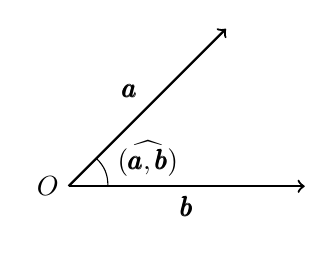
\begin{tikzpicture}
			\node[left] at (0,0){$O$};
			\draw[->, thick] (0,0) -- node[below] {$\pmb{b}$} (3,0); 
			\draw[->, thick] (0,0) -- node[above left] {$\pmb{a}$} (2,2);
			\draw (0.5,0) to[in=315, out=90] (0.354, 0.354);
			\node[right] at (0.5, 0.35){$(\widehat{\pmb{a}, \pmb{b}})$};
		\end{tikzpicture}
	\end{center}
	如果$\pmb{a}$与$\pmb{b}$当中有一个是零向量,那么我们约定$(\widehat{\pmb{a},
	\pmb{b}})$可以取为$[0,\pi]$当中的任意一个值.
	如果两个向量$\pmb{a}$与$\pmb{b}$的夹角是$0$或者$\pi$那么我们就称这两个向量互相{\bf
	平行},记作$\pmb{a}\sslash \pmb{b}$;
	如果两个向量的夹角是$\pi/2$, 那么我们就称这两个向量互相{\bf
	垂直},记作$\pmb{a} \perp \pmb{b}$.
	由于我们规定零向量的方向是任意的,所有零向量与任何向量都垂直,而且与任何向量都
	平行.
\end{definition}

对于多个向量,我们还有共线和共面的关系.  给定$\pmb{a}_1, \pmb{a}_2, \ldots,
\pmb{a}_k$这$k$个向量,如果我们把它们的起点放在一起后它们的终点刚好在同一条直线上面,那么
我们就称$\pmb{a}_1, \pmb{a}_2, \ldots,
\pmb{a}_k${\bf 共线};
同样的道理,如果我们把它们的起点放在一起后它们的终点刚好在同一个平面上,那么
我们就称$\pmb{a}_1, \pmb{a}_2, \ldots,
\pmb{a}_k${\bf 共面}.

\begin{remark}
	两个向量平行当且仅当它们共线.
\end{remark}

接下来我们来复习一下空间当中向量之间的一些常见的运算. 


\begin{definition}
	假设$\pmb{a}$与$\pmb{b}$是两个向量,任取一点$A$并且以$A$为起点作向量$\pmb{a}$, 
	将其终点记作$B$;再以$B$为起点作向量$\pmb{b}$, 将其终点记作$C$,
	那么我们称向量$\overrightarrow{AC}$为向量$\pmb{a}$与$\pmb{b}$的{\bf
	和},并将它记作$\pmb{a}+\pmb{b}$. 如下图所示,$\pmb{a}+\pmb{b}=
	\overrightarrow{AC}$. 
	\begin{center}
		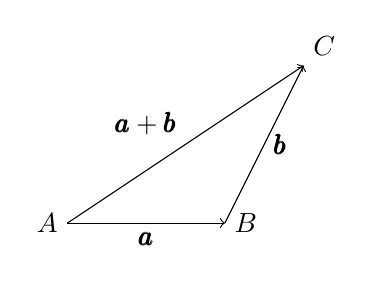
\begin{tikzpicture}
			\node[left] at (0,0) {$A$}; 
			\draw[->] (0,0) -- node[below] {$\pmb{a}$} (2,0)
			node[right] {$B$};
			\draw[->] (2,0) -- node[right] {$\pmb{b}$} (3,2)
			node[above right]{$C$};
			\draw[->] (0,0) -- node[above left] {$\pmb{a}+
			\pmb{b}$} (3,2);
		\end{tikzpicture}
	\end{center}
\end{definition}

上面定义的求和方法称为{\bf 三角形法则}.
我们知道,求向量的和还可以使用所谓的{\bf 平行四边形法则}. 参见下图.

\begin{center}
	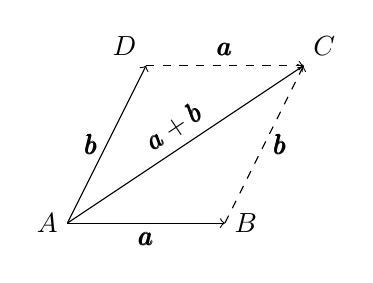
\begin{tikzpicture}
		\node[left] at (0,0) {$A$}; 
		\draw[->] (0,0) -- node[below] {$\pmb{a}$} (2,0)
		node[right] {$B$};
		\draw[->, dashed] (2,0) -- node[right] {$\pmb{b}$} (3,2)
		node[above right]{$C$};
		\draw[->] (0,0) -- node[above, sloped] {$\pmb{a}+
		\pmb{b}$} (3,2);
		\draw[->] (0,0) -- node[left] {$\pmb{b}$} (1,2) node[above
		left] {$D$};
		\draw[->, dashed] (1,2) -- node[above] {$\pmb{a}$} (3,2); 
	\end{tikzpicture}
\end{center}


容易验证,这样定义的向量的加法满足下面的运算规律:

\begin{enumerate}
	\item 交换律:$\pmb{a}+\pmb{b}=\pmb{b}+\pmb{a}$. 
	\item 结合律:$(\pmb{a}+\pmb{b}) + \pmb{c} = \pmb{a}+ (\pmb{b} +
		\pmb{c})$. 
\end{enumerate}

\subsection{作业}
\subsection{教学反思}






\section{一阶线性微分方程}
\subsection{教学目的}
\subsection{教学重点与难点}
\subsection{教学内容与过程}
\subsection{作业}
\subsection{教学反思}






\end{document}



